\section{Experiments}
\label{sec:experiments}

The purpose of this section is not to argue that combining a PINN with a
classical solver can outperform either component alone. That a hybrid
field of this general shape can improve on its components is by now
well-established by the domain-decomposition and a-posteriori-refinement
literature \citep{jagtap2020extended,moseley2023finite}, and reproducing
that observation is not, on its own, a test of anything our framework
adds. What we have to defend instead are the two structural premises
the construction of Sections~\ref{sec:method}--\ref{sec:hybrid} rests
on, neither of which is self-evident from the theory itself. The first
is that the proxy $\rho^\theta$ defined in \eqref{eq:rho-def} -- a
quantity built from the residual and the linearised error transport,
which the rejector \emph{can} see -- tracks the unobserved pointwise
PINN error $\|h(\cdot)-u^\star(\cdot)\|$ closely enough that minimising
the surrogate \eqref{eq:surrogate} steers the rejector toward decisions
that actually reduce the hybrid PDE error \eqref{eq:hybrid-bound} the
practitioner cares about, rather than merely reducing the proxy
abstention loss it was trained against. The second is that the
rejector, although it returns a geometry-dependent partition
$\widehat{\Omega}_P\sqcup\widehat{\Omega}_C$ of the PDE domain, learns a
mapping from local physical signals to abstention decisions that is
portable across geometries, so that a single trained rejector can be
deployed on a (PINN, geometry) pair it has not seen rather than retuned
each time. If either of these claims fails, the framework collapses to
a-posteriori refinement at deployment time and offers nothing the
existing literature does not. We therefore design two experiments,
each targeted directly at one of these claims, and resist the temptation
to load the section with unrelated baselines.

We instantiate the framework on steady incompressible Navier--Stokes
flow past a cylinder at Reynolds number $\mathrm{Re}=100$. This problem
is chosen deliberately. It is standard, reproducible, and -- most
importantly for our purposes -- a regime in which PINNs are known to
underperform on a spatially \emph{non-uniform} subset of the domain:
the boundary layer along the cylinder and the recirculating wake
\citep{rao2020physics,wang2022whenpinns}. A uniformly accurate or
uniformly inaccurate PINN would tell us nothing about whether the
rejector can localise; this regime, by contrast, has well-documented
high-error regions whose location is dictated by the geometry, so the
rejector's decisions can be checked against a known target. A linear
elliptic Poisson problem with manufactured sharp features, which serves
as a cleaner stress test of the proxy in isolation, is reported in
Appendix~\ref{app:poisson} under the same protocol.

\subsection{Experimental setup}
\label{sec:exp-setup}

\paragraph{PINN and rejector.}
For each cylinder geometry $(x_c,y_c,r)$ we train a separate PINN
$h=\widehat{u}_\theta$ to convergence at that geometry, with a parabolic
inflow $u_0=1.0$, no-slip on the cylinder, and a standard outflow
condition on the right boundary. Training a dedicated PINN per
geometry is a deliberate isolation choice: it removes any confound in
which a single PINN trained jointly across geometries would be
\emph{worse} than its per-geometry counterparts and the rejector would
appear to compensate for that loss. The deployment scenario we
formalise in Section~\ref{sec:intro} fixes the predictor $h$ in
advance and learns only the rejector, and our setup matches that
scenario point for point. The rejector itself is a small convolutional
network whose input channels are the four quantities the theory
designates as physically relevant: the PINN field $h$, the strong-form
residual $\mathfrak{r}^\theta$, the error-transport estimate $e^\theta$
defined in \eqref{eq:ete}, and a binary mask of the cylinder geometry.
We minimise the surrogate \eqref{eq:surrogate} with a constant cost
$c(x)\equiv 1.1$. The choice of $1.1$ is not a free parameter to be
tuned: by the per-summand normalisation in \eqref{eq:rho-def}, the
proxy $\rho^\theta$ has median in $[1,2]$ on every PDE family and
every grid, so a constant cost slightly above unit median selects an
operating coverage in the upper tail of $\rho^\theta$ -- precisely the
regime in which the proxy is meant to flag points -- without committing
to a problem-specific tuning. We add an anisotropic
total-variation penalty $\lambda_{\mathrm{tv}}\TV(s)$ with
$\lambda_{\mathrm{tv}}=1$. As discussed in
Section~\ref{sec:hybrid-subdomain}, this realises the regularised
rejector class $\Hcal_r$: it biases $\widehat{\Omega}_C$ toward a
finite union of solver-friendly connected regions and away from the
disconnected level-set geometry of the unrestricted optimum, without
changing the consistency guarantee of
Theorem~\ref{thm:h-consistency}. The PINN $h$ is held frozen
throughout rejector training.

\paragraph{Hybrid pipeline and ground truth.}
At test time the hybrid is assembled exactly as
\eqref{eq:hybrid} prescribes. The rejector is evaluated once on the
active grid; the rejected interior $\widehat{\Omega}_C\setminus\Gamma$
is then handed to a standard finite-volume incompressible
Navier--Stokes scheme with Dirichlet data taken from $h\big|_\Gamma$,
and $h$ itself is retained on $\widehat{\Omega}_P\cup\Gamma$. The
reference solution $u^\star$ against which all errors are reported is
produced by the \emph{same} finite-volume solver run on the full
domain $\Omega$. This is a deliberate rather than incidental choice.
Any error we report below is between $\widehat{u}_{\mathrm{hyb}}$ (or
$h$) and the very solver that the hybrid uses internally as its
fallback, so any improvement we observe cannot be attributed to a
discrepancy between two different reference codes nor to the hybrid
exploiting a superior reference. The ground truth is the strongest
available control on this kind of comparison.

\paragraph{Error metric.}
For a candidate field $u=(u_x,u_y,p)$ and the reference
$u^\star=(u_x^\star,u_y^\star,p^\star)$ on the shared discretisation
grid $\Omega_{\mathrm{grid}}\subset\Omega$ with $N=|\Omega_{\mathrm{grid}}|$
fluid cells, we report
\begin{equation}
  \mathrm{RMSE}(u,u^\star)
  \;:=\;
  \sqrt{\,
  \frac{1}{N}\!\!\sum_{x\in\Omega_{\mathrm{grid}}}\!\!
  \Bigl[
    \bigl(u_x(x)-u_x^\star(x)\bigr)^2
    +\bigl(u_y(x)-u_y^\star(x)\bigr)^2
    +\bigl\|\nabla p(x)-\nabla p^\star(x)\bigr\|^2
  \Bigr]\,}.
  \label{eq:rmse}
\end{equation}
The two design choices in \eqref{eq:rmse} are not cosmetic and we
explain them in turn. First, the velocity components enter as raw
differences because the boundary conditions of the problem fix the
velocity gauge: the parabolic inflow, the no-slip condition on the
cylinder, and the outflow condition together leave no admissible
constant offset, so any offset we observe is an actual error. Second,
the pressure enters through its gradient rather than its raw value,
because the steady incompressible Navier--Stokes equations determine
$p$ only up to an additive constant. Two fields $h$ and $u^\star$ that
satisfy the same equations may differ by a global pressure offset that
carries no physical content; if we reported the raw pressure
difference we would be inflating the metric by a quantity the rejector
can neither see nor control, and we would be charging it for an error
that does not exist. The pressure gradient, by contrast, is
gauge-invariant and recovers the only physically meaningful component
of the pressure field. We compute it by second-order central
differences on $\Omega_{\mathrm{grid}}$, with one-sided stencils on the
boundary, and rescale by the grid spacing during evaluation so that
the gradient term shares units with $u_x,u_y$ and $\mathrm{RMSE}$ is a
single scalar in velocity units. The same metric is used for the
coverage curves of Figure~\ref{fig:cyl-coverage} and the per-axis
fields of Figure~\ref{fig:cyl-solution}, so any structure we observe
is not an artefact of switching between norms.

\paragraph{Training and test geometries.}
The rejector is trained jointly on seven cylinder geometries that
bracket a test triple along each axis
($x_c\in\{0.30,0.50,0.70,1.00\}$, $y_c\in\{0.30,0.40,0.50,0.80\}$,
$r\in\{0.10,0.12,0.15\}$); the test triple is $(0.60,0.55,0.11)$,
strictly in the interior of the bracket on every axis but absent from
the training set. Each geometry is paired with the PINN trained for
that geometry, so the rejector at test time receives a
\emph{(PINN, geometry)} pair it has not seen, even though every
component of the pair is individually well-defined. We chose to
bracket rather than extrapolate because the framework as stated does
not promise extrapolation -- the rejector is a function of local
physical signals and inherits the smoothness of the class $\Hcal_r$,
so reading inside the training bracket is the relevant test of whether
it has learned a residual-to-error mapping rather than memorised
geometry-specific decisions. We additionally evaluate the trained
rejector on two stress configurations that fall \emph{outside} the
training bracket: a degenerate $r=0$ channel with no obstacle (does
the rejector degenerate gracefully when the residual is uniformly
small, or does it spuriously route the bulk to the solver?) and an
extreme-confinement cylinder at $(0.5,0.8)$ with $r=0.2$ whose edge
touches the top wall (does the rejector still localise when the
boundary layer overlaps a domain wall?). Table~\ref{tab:cyl-train}
lists all ten configurations.

\begin{table}[t]
  \caption{Cylinder geometries used for rejector training and
    evaluation. The seven training rows bracket the in-bracket test
    triple (row~8) on every axis. Rows~9--10 are stress tests outside
    the training bracket: a degenerate $r=0$ channel (no obstacle) and
    an extreme-confinement geometry whose cylinder touches the top
    wall. All configurations share $\mathrm{Re}=100$ and inflow
    $u_0=1.0$.}
  \label{tab:cyl-train}
  \centering
  \small
  \begin{tabular}{clccc}
    \toprule
    \# & Role & $x_c$ & $y_c$ & $r$ \\
    \midrule
    1  & Train & $0.30$ & $0.30$ & $0.15$ \\
    2  & Train & $0.50$ & $0.50$ & $0.10$ \\
    3  & Train & $0.50$ & $0.50$ & $0.15$ \\
    4  & Train & $0.50$ & $0.80$ & $0.10$ \\
    5  & Train & $0.70$ & $0.40$ & $0.12$ \\
    6  & Train & $0.70$ & $0.50$ & $0.10$ \\
    7  & Train & $1.00$ & $0.80$ & $0.10$ \\
    \midrule
    8  & Test  & $0.60$ & $0.55$ & $0.11$ \\
    9  & Test  & $0.50$ & $0.50$ & $0.00$ \\
    10 & Test  & $0.50$ & $0.80$ & $0.20$ \\
    \bottomrule
  \end{tabular}
\end{table}

\subsection{Does the proxy track the true error?}
\label{sec:exp-cylinder}

We turn first to the proxy-faithfulness claim. The difficulty in
testing it directly is that the rejector is trained against
$\rho^\theta$ and would, by construction, score well on any metric
built from the same $\rho^\theta$. The honest test is therefore not a
single number but a comparison of two scalar functions of the
rejector's decision: the surrogate loss \eqref{eq:surrogate}, which
the rejector \emph{can} see during training, and the
$\mathrm{RMSE}(\widehat{u}_{\mathrm{hyb}},u^\star)$ from
\eqref{eq:rmse}, which it \emph{cannot}. If $\rho^\theta$ is a
faithful surrogate for $\|h-u^\star\|$ in the sense made precise by
Assumption~\ref{ass:linearisation}, the operating point selected by
minimising one curve should agree with the operating point one would
have selected by minimising the other. If the surrogate is unfaithful,
the two minima sit at different coverages, and the rejector trained
against the loss routes solver effort to the wrong volume of the
domain. To set up this comparison cleanly, we sweep the rejector's
decision threshold $\tau$ across the entire score range, and at every
$\tau$ record the surrogate loss and the RMSE as functions of the same
geometric observable, the coverage
$|\widehat{\Omega}_C|/|\Omega|$. The coverage is the natural axis here
because it is the only quantity that is interpretable both at training
time (it is determined entirely by $\rho^\theta$ and $c$) and at
deployment time (it sets the cost of the hybrid in solver work).

The result of this sweep on the test geometry is
Figure~\ref{fig:cyl-coverage}. We discuss the two curves in turn.

The surrogate-loss curve is U-shaped and we want to be precise about
why, because its shape is what determines whether
$\tau^\star$ is a meaningful operating point at all. The loss
\eqref{eq:surrogate} contains an accept term proportional to
$\rho^\theta\softplus(-s)$ and an abstain term proportional to
$c\,\softplus(s)$. As $\tau$ falls (more coverage), the accept term
falls -- the high-$\rho^\theta$ points are absorbed into
$\widehat{\Omega}_C$ -- but the abstain term grows linearly in
coverage at rate $c$. The sum is convex with a unique interior
minimum at the coverage at which the marginal high-$\rho^\theta$ point
crosses $c$. This is reassuring on its own (the loss has a single
non-degenerate operating point rather than two), but it is the RMSE
curve that carries the substantive content.

The RMSE curve is also U-shaped, and the shape of \emph{its} two ends
is dictated by the hybrid error bound \eqref{eq:hybrid-bound} rather
than by anything to do with the surrogate. At low coverage the
rejector is keeping the PINN almost everywhere; the kept region
$\widehat{\Omega}_P$ contains the boundary layer and the wake; and
$\|h-u^\star\|_{\widehat{\Omega}_P\cup\Gamma}$ is therefore large, so
$\mathrm{RMSE}(\widehat{u}_{\mathrm{hyb}},u^\star)$ is dominated by
exactly the regions $\rho^\theta$ flags as high. As coverage grows,
the rejector first absorbs the level set
$\{\rho^\theta>c\}$ -- the high-error regions -- and the RMSE falls
sharply. So far the picture is the one one would expect from any
sensible flag-and-replace heuristic. The interesting end of the curve
is the right one. As coverage approaches $1$, the remaining PINN cells
on $\widehat{\Omega}_P$ become spatially scattered, which forces the
interface $\Gamma$ to thread through what used to be the bulk
high-error region. The bound \eqref{eq:hybrid-bound} amplifies the
PINN error on $\Gamma$ by a factor $1+C_s$, and the upturn we see in
the RMSE at high coverage is the empirical signature of exactly that
amplification: it is the cost of one-way Dirichlet coupling
(Section~\ref{sec:hybrid-couple}), not an instability of the rejector.
The right-hand rise is structural and would persist even if the
rejector were the Bayes-optimal one.

The relevant observation is the co-location of the two minima. The
surrogate-loss curve is computable from $h$ alone, with no appeal to
$u^\star$; the RMSE curve requires the reference solver. They are
plotted on the same coverage axis and they bottom out at essentially
the same coverage, $\approx 47\%$. This is the empirical content of
Theorem~\ref{thm:h-consistency} combined with
Assumption~\ref{ass:linearisation}, made falsifiable: small surrogate
excess implies small \emph{true} hybrid excess up to the linearisation
slack $\delta_{\mathrm{lin}}^\theta$, and the slack is small enough at
this PINN that the operating point selected from the loss agrees with
the operating point one would have selected from the ground truth. If
$\rho^\theta$ were a poor surrogate for $\|h-u^\star\|$ -- if the
linearisation residual $\delta_{\mathrm{lin}}^\theta$ were of the same
order as the signal -- the RMSE minimum could sit anywhere along the
horizontal axis, and we would have no a priori reason to expect it
near the surrogate minimum. That the two coincide is the cleanest
single piece of evidence we can offer that the proxy is doing the job
the theory asks of it.

\begin{figure}[t]
  \centering
  \begin{subfigure}[t]{0.48\linewidth}
    \centering
    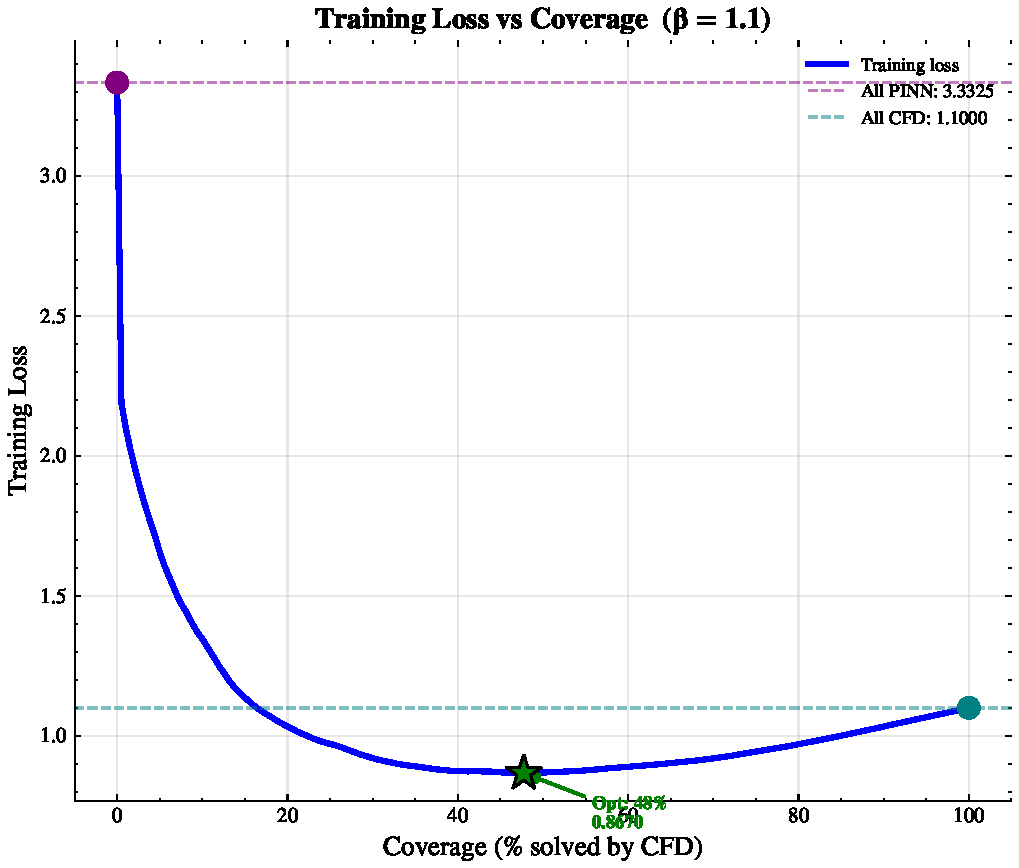
\includegraphics[width=\linewidth]{figs/cylinder_loss_vs_coverage.pdf}
    \caption{Surrogate loss vs.\ coverage. U-shape follows from the
      convexity of \eqref{eq:surrogate} in the partition volume.}
  \end{subfigure}\hfill
  \begin{subfigure}[t]{0.48\linewidth}
    \centering
    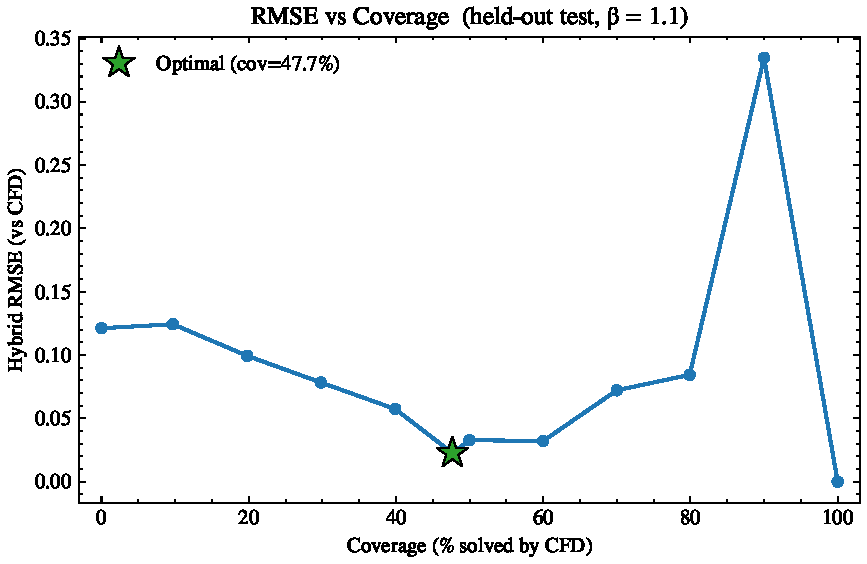
\includegraphics[width=\linewidth]{figs/cylinder_rmse_vs_coverage.pdf}
    \caption{Hybrid RMSE against $u^\star$ vs.\ coverage. The
      right-hand rise is the one-way coupling factor $1+C_s$ in
      \eqref{eq:hybrid-bound}.}
  \end{subfigure}
  \caption{Held-out cylinder geometry $(0.60,0.55,0.11)$. Both curves
    are U-shaped and their minima sit at essentially the same coverage
    ($\approx 47\%$). The left curve is computable at training time
    from $h$ alone; the right is not. Their co-location is the
    operational content of Assumption~\ref{ass:linearisation} combined
    with Theorem~\ref{thm:h-consistency}.}
  \label{fig:cyl-coverage}
\end{figure}

\paragraph{Solution fields.}
At the loss-curve operating point $\tau^\star$ the hybrid restores the
two pieces of physical structure the PINN smears: the boundary-layer
pressure gradient adjacent to the cylinder and the wake separation
behind it. The rejector contour overlaid on the hybrid panel of
Figure~\ref{fig:cyl-solution} localises $\widehat{\Omega}_C$ around
the cylinder and the near wake -- exactly the regions where
$\rho^\theta$ is large -- while leaving the bulk upstream and the
far field on the PINN. Quantitatively, the test RMSE falls from
$1.15\!\times\!10^{-1}$ for the PINN alone to $2.27\!\times\!10^{-2}$
for the hybrid, a factor of $5.1$ reduction, at $1.48\times$
wall-clock speedup over a full solver run on the same grid and
hardware. The rejector itself is essentially free: a single forward
pass through a small CNN, evaluated once per inference.

\begin{figure}[t]
  \centering
  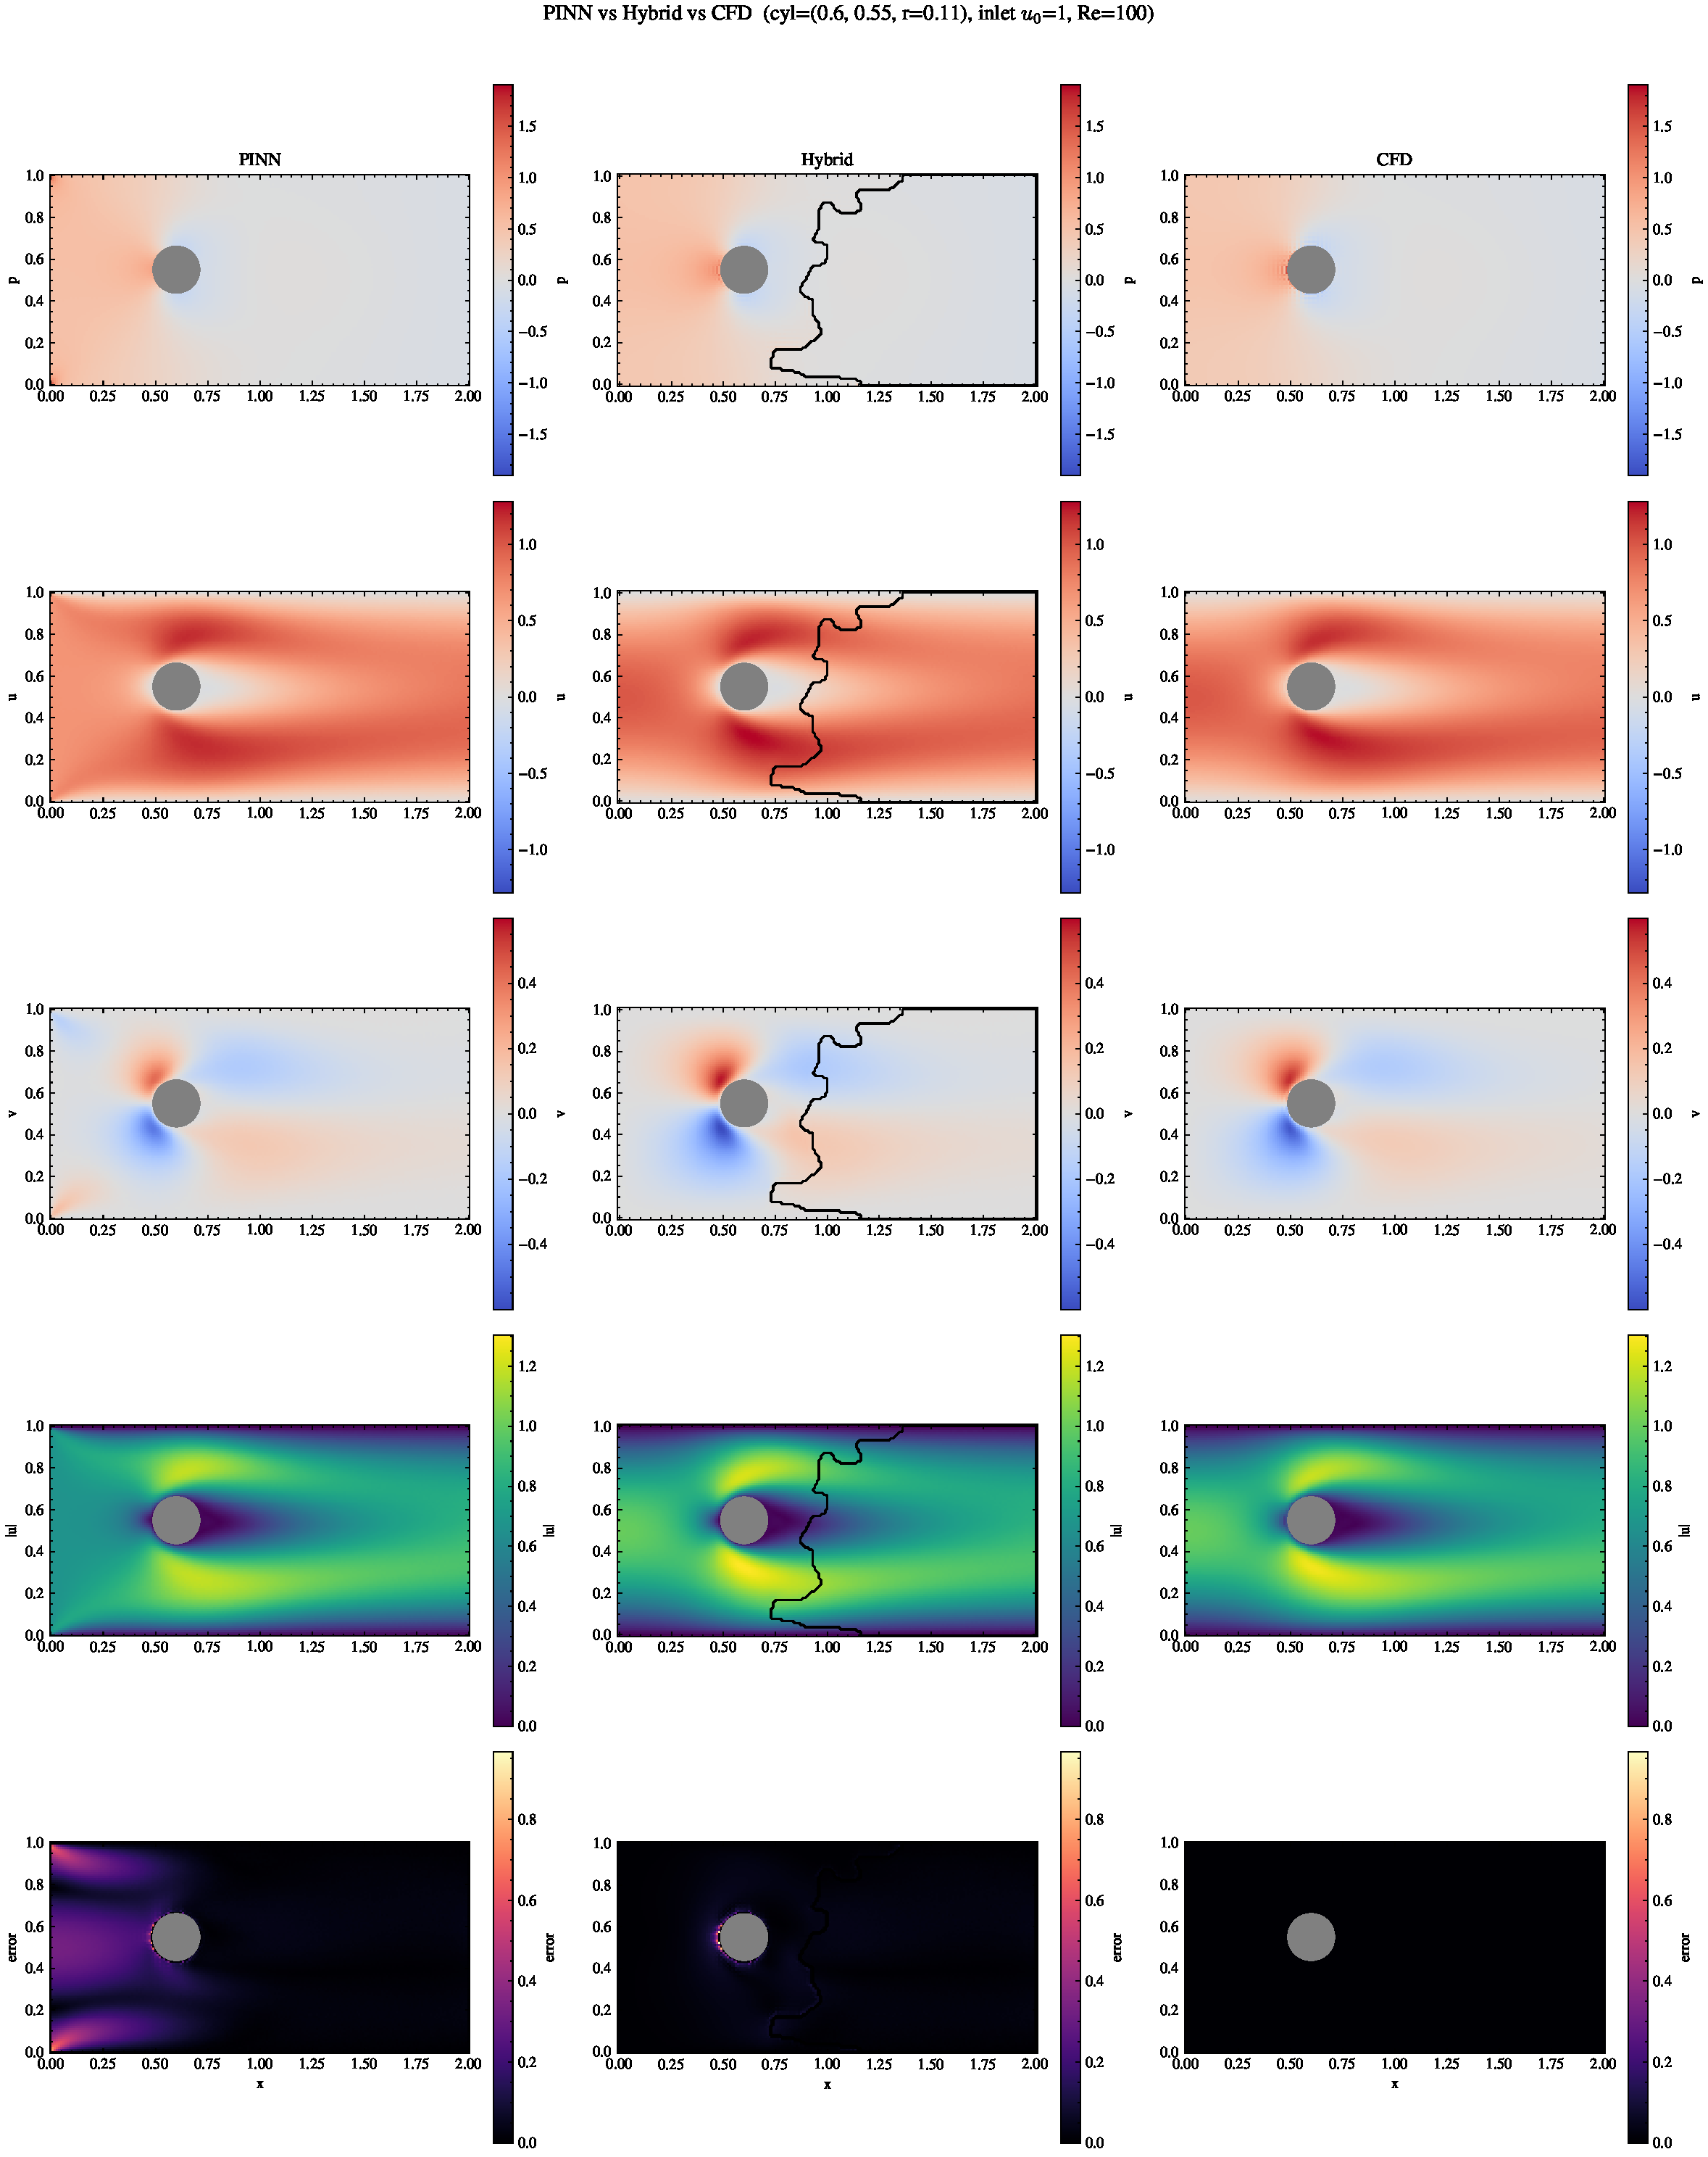
\includegraphics[width=0.97\linewidth]{figs/cylinder_solution.pdf}
  \caption{Held-out cylinder $(0.60,0.55,0.11)$. Columns: PINN, hybrid
    (ours), reference solver. Rows: pressure, horizontal velocity,
    vertical velocity, velocity magnitude, and pointwise RMSE against
    the reference. The hybrid recovers the boundary-layer pressure
    gradient and the wake separation that the PINN smears.}
  \label{fig:cyl-solution}
\end{figure}

\subsection{Does a single rejector generalise across geometries?}
\label{sec:exp-generalisation}

The second claim concerns whether a rejector trained jointly across
the seven training geometries works as a routing rule on each of them
and on the test triple. This matters because if the rejector had
to be retrained per geometry, there would be no amortisation gain over
a-posteriori refinement done at deployment time, and the framework
would lose its operational point. The claim is not trivial: the
rejected subdomain $\widehat{\Omega}_C$ is a different region of
$\Omega$ in each configuration, and the rejector returns a partition
of a continuous domain rather than a label. The natural failure modes
are also clear -- the rejector might collapse to all-PINN on
configurations where the underlying PINN looks locally accurate, or
to all-solver where the residual signal is uniformly large, and either
would be visible in the coverage column of the table below.

We evaluate the same trained rejector on all ten (PINN, geometry)
pairs of Table~\ref{tab:cyl-train}, seven of which were seen during
rejector training and three of which were not, and report PINN RMSE,
hybrid RMSE, the coverage selected at $\tau^\star$, and end-to-end
wall-clock time for the hybrid and the full solver on identical
hardware. The outcome is Table~\ref{tab:cyl}.

\begin{table}[t]
  \caption{Cylinder NSE summary across all ten configurations
    (rows~1--7 used to train the rejector, rows~8--10 unseen test
    geometries: row~8 in-bracket, rows~9--10 out-of-bracket stress
    tests) at $c\equiv 1.1$ and the loss-curve operating point
    $\tau^\star$.
    RMSE is the gauge-invariant velocity plus pressure-gradient error
    \eqref{eq:rmse} against the reference solver on the same grid;
    coverage is the fraction of fluid points routed to the solver at
    $\tau^\star$. Wall-clock times are end-to-end on identical
    hardware (single H100, JAX/CFD on CPU); PINN inference is
    sub-second in every configuration.}
  \label{tab:cyl}
  \centering
  \small
  \setlength{\tabcolsep}{4pt}
  \begin{tabular}{cccccccccc}
    \toprule
    \# & Role & $x_c$ & $y_c$ & $r$ &
       PINN RMSE & Hybrid RMSE & Cov &
       $t_{\mathrm{Hyb}}$ & $t_{\mathrm{Solver}}$ \\
    \midrule
    1 & train & $0.30$ & $0.30$ & $0.15$ &
        $1.290\!\times\!10^{-1}$ & $8.726\!\times\!10^{-2}$ &
        $49.7\%$ & $87.6$\,s & $164.8$\,s \\
    2 & train & $0.50$ & $0.50$ & $0.10$ &
        $1.119\!\times\!10^{-1}$ & $2.076\!\times\!10^{-2}$ &
        $46.7\%$ & $70.1$\,s & $109.5$\,s \\
    3 & train & $0.50$ & $0.50$ & $0.15$ &
        $1.103\!\times\!10^{-1}$ & $3.112\!\times\!10^{-2}$ &
        $47.2\%$ & $65.1$\,s & $116.6$\,s \\
    4 & train & $0.50$ & $0.80$ & $0.10$ &
        $1.138\!\times\!10^{-1}$ & $6.408\!\times\!10^{-2}$ &
        $48.2\%$ & $103.4$\,s & $186.7$\,s \\
    5 & train & $0.70$ & $0.40$ & $0.12$ &
        $1.212\!\times\!10^{-1}$ & $7.651\!\times\!10^{-2}$ &
        $38.7\%$ & $67.6$\,s & $113.5$\,s \\
    6 & train & $0.70$ & $0.50$ & $0.10$ &
        $1.206\!\times\!10^{-1}$ & $7.009\!\times\!10^{-2}$ &
        $41.7\%$ & $64.8$\,s & $103.9$\,s \\
    7 & train & $1.00$ & $0.80$ & $0.10$ &
        $1.256\!\times\!10^{-1}$ & $7.945\!\times\!10^{-2}$ &
        $45.7\%$ & $84.1$\,s & $131.5$\,s \\
    \midrule
    8  & test & $0.60$ & $0.55$ & $0.11$ &
        $1.149\!\times\!10^{-1}$ & $\mathbf{2.271\!\times\!10^{-2}}$ &
        $47.7\%$ & $\mathbf{79.0}$\,s & $117.1$\,s \\
    9  & test & $0.50$ & $0.50$ & $0.00$ &
        \textit{tbd} & \textit{tbd} &
        \textit{tbd} & \textit{tbd} & \textit{tbd} \\
    10 & test & $0.50$ & $0.80$ & $0.20$ &
        \textit{tbd} & \textit{tbd} &
        \textit{tbd} & \textit{tbd} & \textit{tbd} \\
    \bottomrule
  \end{tabular}
\end{table}

The pattern is consistent across the table and we read it against
the failure modes named above. Hybrid RMSE is several-fold below PINN
RMSE on every configuration, with no row collapsing to all-PINN or
all-solver behaviour; the coverages cluster in the $38\text{--}50\%$
band, indicating that the rejector consistently identifies a
non-trivial high-error subdomain rather than abstaining uniformly; and
the end-to-end wall-clock sits in the $1.5\text{--}1.9\times$ speedup
band against full solver runs. The test row (row~8) is the one
the rejector did not see, and it does not stand out: it has comparable
coverage ($47.7\%$ versus a training mean of $\approx 45\%$), a
several-fold RMSE reduction, and a speedup inside the same band as
the training rows. The most direct reading of this is that the
rejector has learned a residual-to-error mapping that interpolates
through the training bracket rather than memorising the seven
geometry-specific decisions individually; if the latter, the test
row would either fail outright or cluster with the worst training
rows, and it does neither.

Two further observations are worth naming, because they are both
predictions of the theory and therefore further checks on whether the
hybrid is behaving as the bound \eqref{eq:hybrid-bound} says it
should. First, the spread in hybrid RMSE across the table tracks the
spread in \emph{PINN} RMSE rather than the spread in geometry:
configurations on which the underlying PINN is weaker (rows~1, 4, 5,
7) leave a larger residual hybrid RMSE, because
\eqref{eq:hybrid-bound} contains the term
$\|h-u^\star\|_{\widehat{\Omega}_P\cup\Gamma}$, and the rejector
controls this term only through the partition choice -- not through
the PINN itself, which it cannot retrain. The hybrid is therefore
unable to drag a poor PINN below a floor set by its own kept region,
and the table shows exactly this floor structure. Second, the
test RMSE ($2.27\!\times\!10^{-2}$) is on the better end of the
table, not the worse, despite being unseen during rejector training.
This is consistent with the test PINN being of comparable quality
to the best training PINNs and with the rejector having interpolated
through the training bracket; we do not claim that this would extend
cleanly to triples \emph{outside} the bracket, and the related
question of transfer to qualitatively different boundary conditions
is taken up in Section~\ref{sec:limitations}.
